\documentclass[11pt]{article} %original font size 11

% Change "review" to "final" to generate the final (sometimes called camera-ready) version.
% Change to "preprint" to generate a non-anonymous version with page numbers.
\usepackage[preprint]{acl}

% Standard package includes
\usepackage{times}
\usepackage{latexsym}

% For proper rendering and hyphenation of words containing Latin characters (including in bib files)
\usepackage[T1]{fontenc}

% This assumes your files are encoded as UTF8
\usepackage[utf8]{inputenc}

\usepackage{microtype}
\usepackage{graphicx}
\usepackage{booktabs}
\usepackage{tabularx}
\usepackage{xcolor}
\usepackage{hyperref}

\definecolor{primary}{RGB}{30, 41, 59}
\definecolor{secondary}{RGB}{71, 85, 105}
\definecolor{accent}{RGB}{2, 132, 199}

\hypersetup{colorlinks=true, linkcolor=accent, urlcolor=accent}

\title{Analyzing Cross-Lingual Topic Spaces and Story Representations in Pre-Trained
Language Models}

\author{Luc De Nardi \\ University of Colorado, Boulder \\ \texttt{denardiluc@gmail.com}}

\begin{document}
    \maketitle

    \section{Introduction}
    Storytelling is an inherently human creation brings communities together. Culture
    can be ingrained into these stories. Pre-trained models are good at taking
    in high resource languages and finding topics, this could be seen as a double
    sided sword when it comes to low/medium resourced languages. I tested
    whether three popular models can agree on topics from several low and medium
    resource languages. If we have models be trained on more languages there might
    be more representation on cultures which hopefully hopefully steer to less biased
    summarization/aid in better translation.

    With these models, there will be biases from the languages with more data, so
    my main research question is How close are the topics of stories and spoken narratives
    from differing communities of low/medium resourced languages? I hypothesized
    that the topics will be similar by language families and will see pockets in
    the overall space.

    \section{Related work}
    \citet{conneau2020emerging} shows that pretraining multilingual language models
    will lead to higher performance gains for a wide range of cross-lingual transfer
    tasks. \citet{conneau2020emerging} develped the XLM-R which is the bases of the
    XLM-RoBerta \citep{DBLP:journals/corr/abs-1911-02116}. \citet{conneau2020emerging}
    attempted to improve the cross-lingual language understanding (XLU) of the
    models. They did this by carefully studying the effects of the unspervised crosslingual
    training representations at a very large scale.

    \citet{eldan2023tinystories} shows that models around 125 million parameters
    can rarely generate coherent and consistent English text beyond a few words
    even after extensive training. They have produced the TinyStories dataset which
    is a synthetic dataset of short stories which uses words which is typical for
    a 3 to 4-year-olds. These stories were generated by GPT-3.5 and GPT-4. These
    stories can be used to train and evaluate models that are much smaller than
    the state-of-the-art models.

    \citet{adelani-etal-2022-masakhanews} has developed MasakhaNEWS which is the largest
    dataset for news topic classification. This dataset covers 16 languages
    widely spoken in Africa. This dataset has shaped how the development of several
    machine learning algorithms have been done, such as topic modeling.

    \citet{bianchi-etal-2021-cross} has shown that many datasets co-exist in multiple
    languages. This covers the same content across the board. \citet{bianchi-etal-2021-cross}
    states that the linguistic differences in the datasets would make it
    impossible to use the more conventional and traditional, bag-of-word-based topic
    models. This is due to the struggles with cross-lingual applications due to
    the sparse vocabulary that some of the datasets provide with just
    monolingual corpora differences. \citet{bianchi-etal-2021-cross} states that
    models can take 2 form, either be monolingual or suffer from a sparse vocabulary
    wich can be troublesome when we want to do multilingual tasks. Transfer
    learning can play a role in mitigating this risk. \citet{bianchi-etal-2021-cross}
    introduces a zero-shot cross-lingual topic model that learns topics in
    English, and predicts them in documents in Italian, French, German, and
    Portuguese. This relates to this project by having a way to do multilingual zero-shot
    models. I am adding the option for low-resource languages and story telling
    to the mix.

    \section{Methodology}
    I have testing on three different models, two are from the Bert family: XLM-RoBERTa
    base \citep{DBLP:journals/corr/abs-1911-02116} and DeBerta v3 Base \citep{he2021debertav3, he2021deberta}
    and a Qwen2.5-7B Instruct \citep{qwen2.5, qwen2} model.

    \section{Data}

    \section{Feasible tests}

    \section{Results}

    \appendix
    \section{Figures and Tables}
    Refer to \autoref{tab:silhouette_scores} to \ref{tab:xlmr_sim} for the tables
    and \autoref{fig:embedd} and \ref{lda} for the two figures.
    \begin{table}[htbp]
        \centering
        \vspace{0.5em}
        \small
        \begin{tabular}{lccc}
            \toprule \textbf{Language} & \textbf{DeBERTa} & \textbf{Qwen} & \textbf{XLM-RoBERTa} \\
            \midrule Acholi            & 0.1994           & 0.0989        & 0.0438               \\
            Luganda                    & 0.1933           & 0.1253        & 0.0853               \\
            Masaaba                    & 0.1800           & 0.0817        & 0.0814               \\
            Nyankole                   & 0.1924           & 0.1210        & 0.0865               \\
            Soga                       & 0.1911           & 0.1170        & 0.0946               \\
            Akan                       & 0.1891           & 0.1277        & 0.0651               \\
            Ewe                        & 0.1813           & 0.0633        & 0.0527               \\
            Dagbani                    & 0.2281           & 0.0730        & 0.0509               \\
            Norwegian                  & 0.1251           & 0.0663        & 0.0744               \\
            Slovak                     & 0.1232           & 0.0656        & 0.0751               \\
            Serbian                    & 0.1313           & 0.1568        & 0.1456               \\
            Bulgarian                  & 0.1145           & 0.0710        & 0.0636               \\
            Czech                      & 0.1216           & 0.0634        & 0.0741               \\
            Turkish                    & 0.1389           & 0.0700        & 0.0819               \\
            Persian                    & 0.1374           & 0.0818        & 0.0657               \\
            Vietnamese                 & 0.1361           & 0.0614        & 0.0720               \\
            Indonesian                 & 0.0958           & 0.0566        & 0.0727               \\
            Assamese                   & 0.1815           & 0.0419        & 0.0648               \\
            Dogri                      & 0.1576           & 0.0957        & 0.0506               \\
            GOM                        & 0.1757           & 0.0730        & 0.0554               \\
            Kannada                    & 0.1461           & 0.0429        & 0.1174               \\
            Nepali                     & 0.1900           & 0.0551        & 0.0296               \\
            Tamil                      & 0.1330           & 0.0468        & 0.0689               \\
            Sindhi                     & 0.1466           & 0.0534        & 0.0461               \\
            \bottomrule
        \end{tabular}
        \caption{Silhouette Scores per Language Across Models}
        \label{tab:silhouette_scores}
    \end{table}

    \begin{table}[htbp]
        \centering
        \small
        \begin{tabular}{llcc}
            \toprule \textbf{Language 1} & \textbf{Language 2} & \textbf{Mean Cosine Sim.} \\
            \midrule Acholi              & Luganda             & 0.9508                    \\
            Acholi                       & Masaaba             & 0.9619                    \\
            Acholi                       & Nyankole            & 0.9583                    \\
            Acholi                       & Soga                & 0.9615                    \\
            Acholi                       & Akan                & 0.9490                    \\
            Acholi                       & Ewe                 & 0.9513                    \\
            Acholi                       & Dagbani             & 0.9727                    \\
            Acholi                       & Norwegian           & 0.6627                    \\
            Acholi                       & Slovak              & 0.6109                    \\
            Acholi                       & Serbian             & 0.6337                    \\
            Acholi                       & Bulgarian           & 0.5994                    \\
            Acholi                       & Czech               & 0.5950                    \\
            Acholi                       & Turkish             & 0.6592                    \\
            Acholi                       & Persian             & 0.7178                    \\
            Acholi                       & Vietnamese          & 0.4640                    \\
            Acholi                       & Indonesian          & 0.6435                    \\
            Acholi                       & Assamese            & 0.7712                    \\
            Acholi                       & Dogri               & 0.8890                    \\
            Acholi                       & GOM                 & 0.9279                    \\
            Acholi                       & Kannada             & 0.7280                    \\
            Acholi                       & Nepali              & 0.7242                    \\
            Acholi                       & Tamil               & 0.7609                    \\
            Acholi                       & Sindhi              & 0.7811                    \\
            Luganda                      & Nyankole            & 0.9677                    \\
            Luganda                      & Soga                & 0.9679                    \\
            Norwegian                    & Slovak              & 0.9842                    \\
            Norwegian                    & Serbian             & 0.9835                    \\
            Slovak                       & Czech               & 0.9935                    \\
            Kannada                      & Nepali              & 0.9748                    \\
            Nepali                       & Sindhi              & 0.9694                    \\
            \bottomrule
        \end{tabular}
        \caption{Cross-Lingual Cosine Similarity Metrics (DeBERTa Model)}
        \label{tab:deberta_sim}
    \end{table}

    \begin{table}[htbp]
        \centering
        \small
        \begin{tabular}{llcc}
            \toprule \textbf{Language 1} & \textbf{Language 2} & \textbf{Mean Cosine Sim.} \\
            \midrule Acholi              & Luganda             & 0.9033                    \\
            Acholi                       & Masaaba             & 0.8999                    \\
            Acholi                       & Nyankole            & 0.9018                    \\
            Acholi                       & Soga                & 0.9156                    \\
            Acholi                       & Akan                & 0.8560                    \\
            Acholi                       & Norwegian           & 0.5413                    \\
            Acholi                       & Bulgarian           & -0.1191                   \\
            Acholi                       & Persian             & -0.1207                   \\
            Acholi                       & Kannada             & -0.0689                   \\
            Luganda                      & Nyankole            & 0.9606                    \\
            Norwegian                    & Slovak              & 0.4964                    \\
            Slovak                       & Czech               & 0.8998                    \\
            Dogri                        & GOM                 & 0.9543                    \\
            Kannada                      & Tamil               & 0.5917                    \\
            \bottomrule
        \end{tabular}
        \caption{Cross-Lingual Cosine Similarity Metrics (Qwen Model)}
        \label{tab:qwen_sim}
    \end{table}

    \begin{table}[htbp]
        \centering
        \small
        \begin{tabular}{llcc}
            \toprule \textbf{Language 1} & \textbf{Language 2} & \textbf{Mean Cosine Sim.} \\
            \midrule Acholi              & Luganda             & 0.9965                    \\
            Acholi                       & Masaaba             & 0.9962                    \\
            Acholi                       & Nyankole            & 0.9967                    \\
            Acholi                       & Norwegian           & 0.9894                    \\
            Luganda                      & Nyankole            & 0.9971                    \\
            Norwegian                    & Slovak              & 0.9974                    \\
            Slovak                       & Czech               & 0.9987                    \\
            Vietnamese                   & Indonesian          & 0.9983                    \\
            Dogri                        & GOM                 & 0.9980                    \\
            Kannada                      & Tamil               & 0.9975                    \\
            \bottomrule
        \end{tabular}
        \caption{Cross-Lingual Cosine Similarity Metrics (XLM-RoBERTa Model)}
        \label{tab:xlmr_sim}
    \end{table}

    \begin{figure*}[t]
        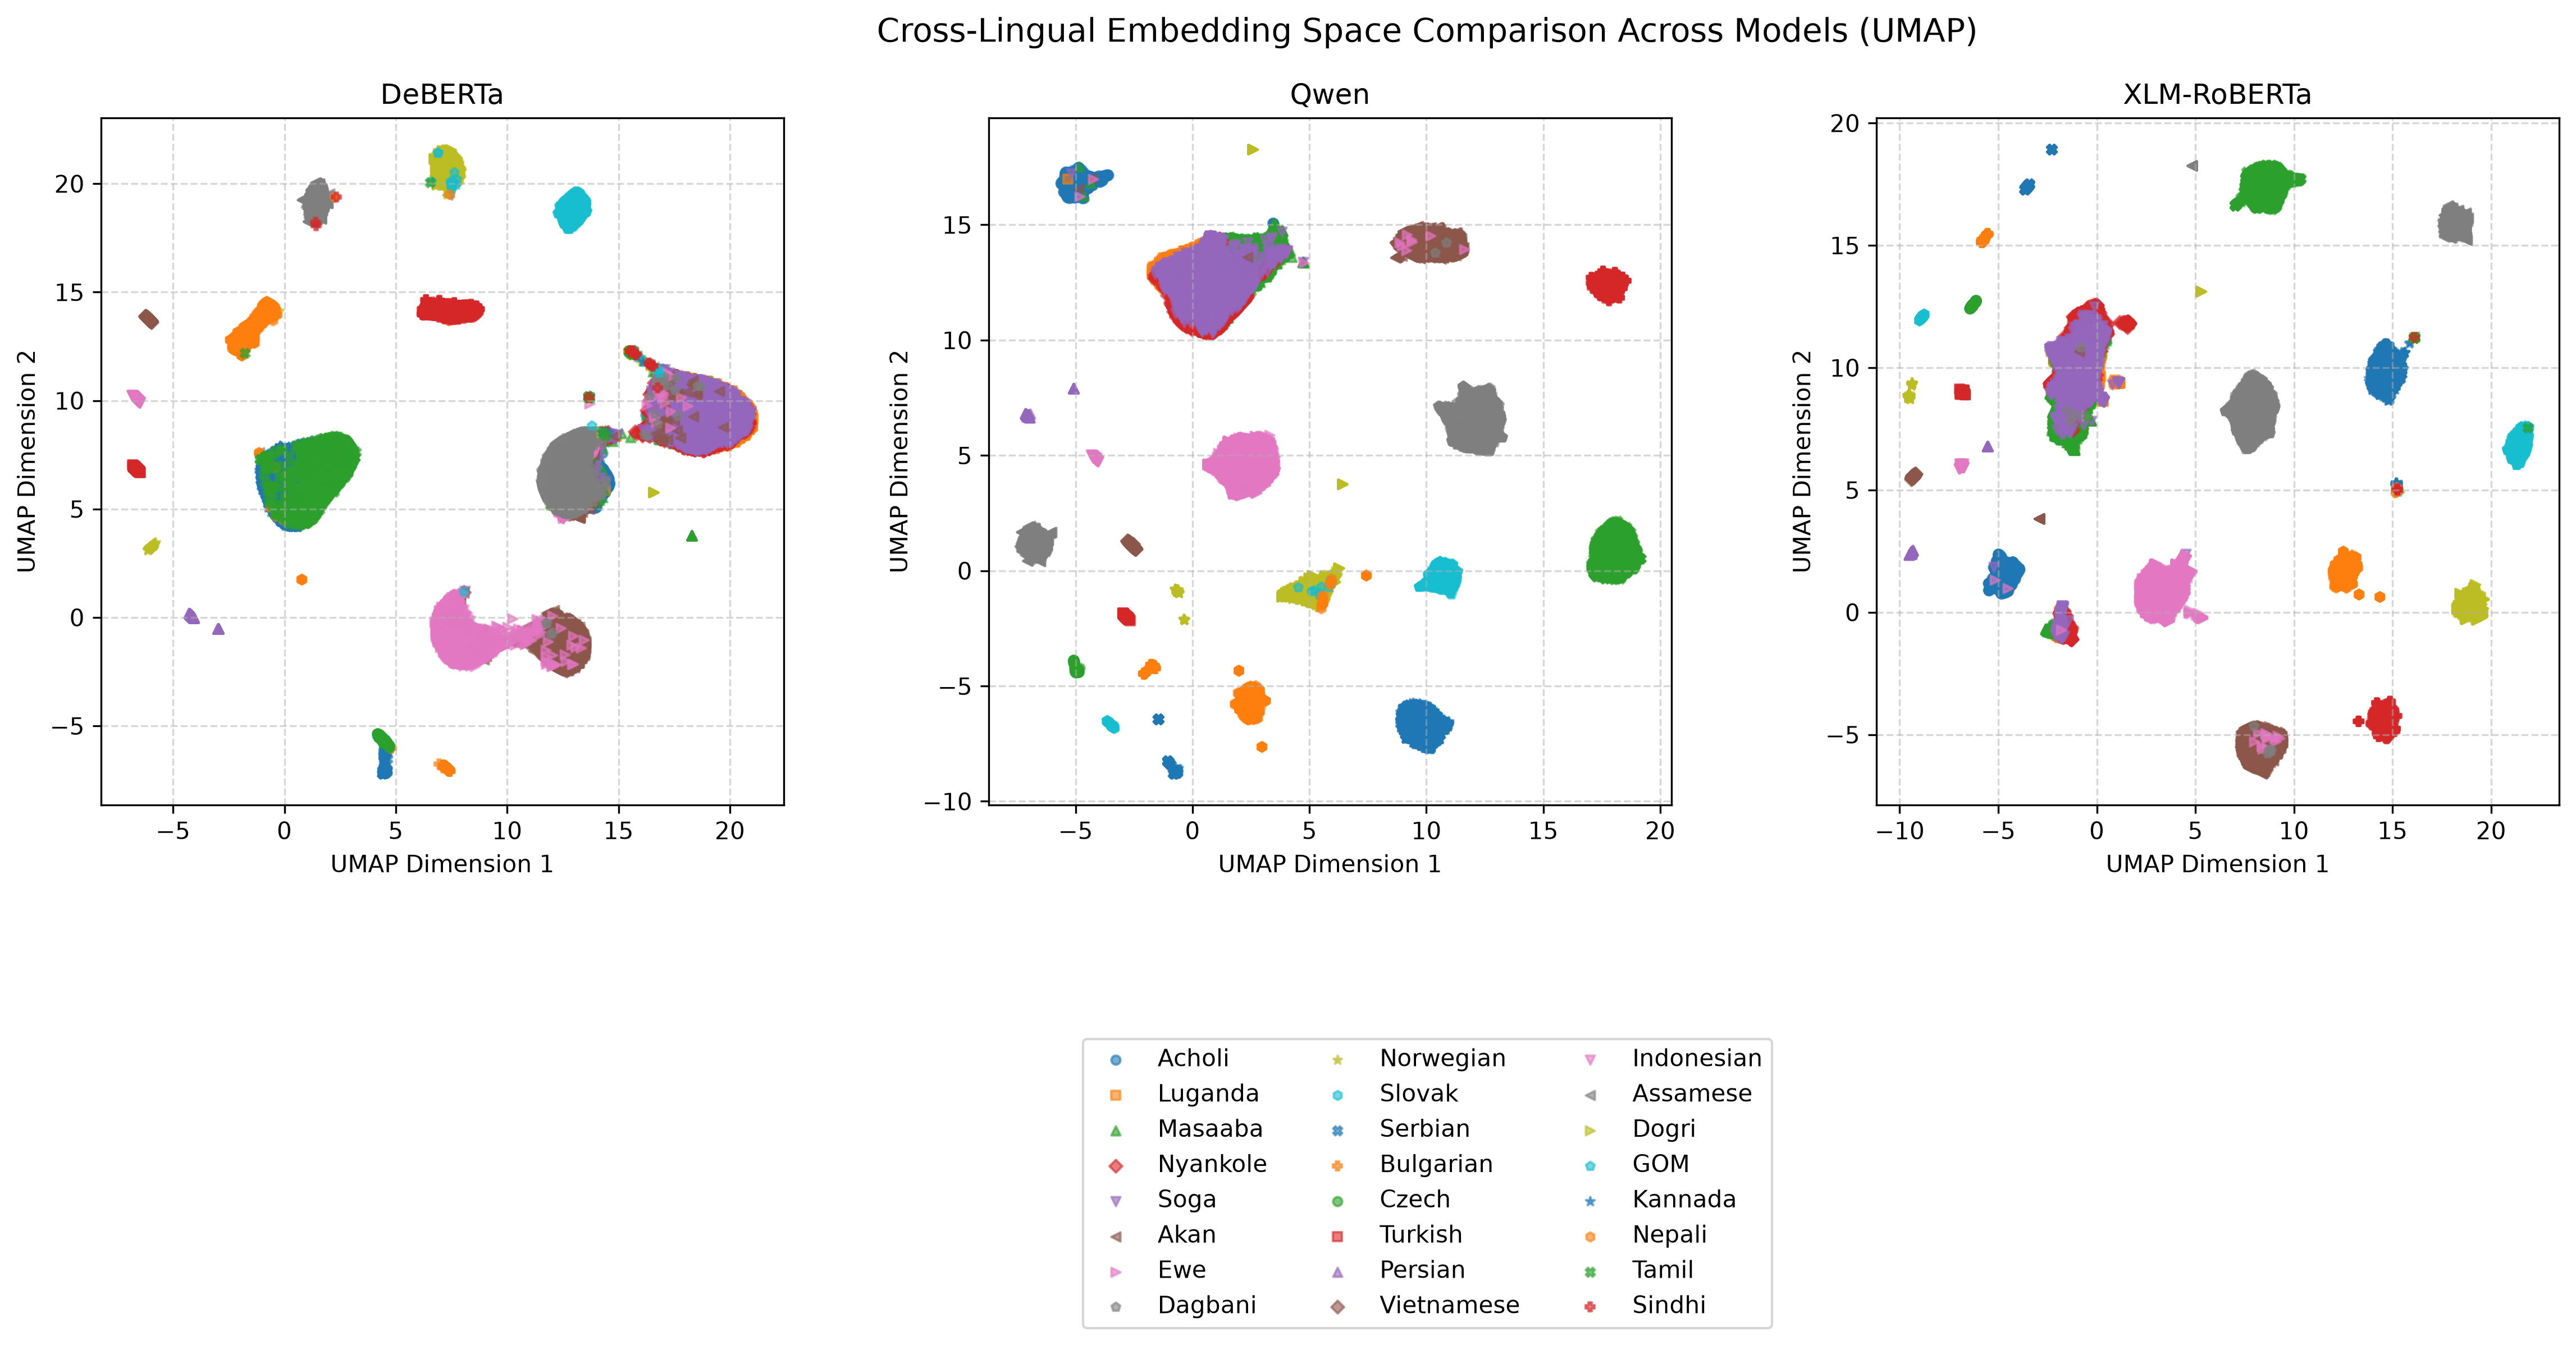
\includegraphics[width=\linewidth]{
            multilingual_models_embedding_space.png
        }
        \caption{A minimal working example to demonstrate how to place two
        images side-by-side.}
        \label{fig:embedd}
    \end{figure*}

    \begin{figure*}[t]
        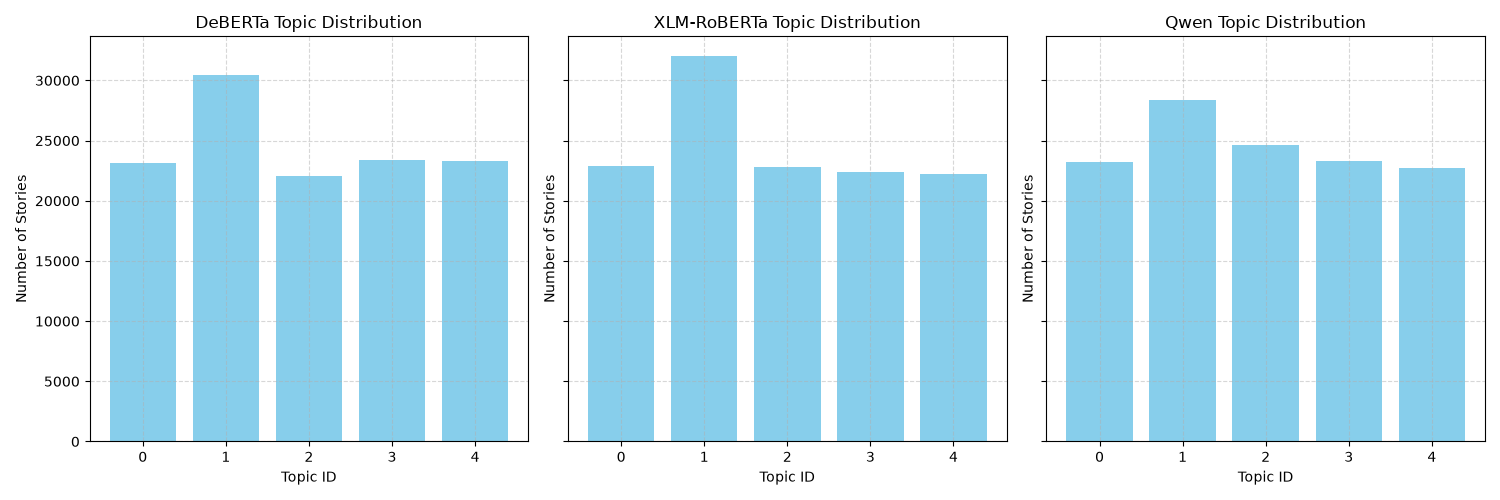
\includegraphics[width=\linewidth]{lda_topic_dist.png}
        \caption{LDA topic categorization distribution}
        \label{lda}
    \end{figure*}

    \begin{table*}
        [t]
        \centering
        \begin{tabular}{lllrrr}
            \toprule   & Language   & Comparison             & Dimension 1 & Dimension 2 & Dimension 3 \\
            \midrule 0 & Acholi     & DeBERTa vs Qwen        & 0.999996    & 0.994984    & 0.996444    \\
            1          & Acholi     & DeBERTa vs XLM-RoBERTa & 0.996180    & 0.983579    & 0.979210    \\
            2          & Luganda    & DeBERTa vs Qwen        & 0.997958    & 0.996214    & 0.992004    \\
            3          & Luganda    & DeBERTa vs XLM-RoBERTa & 0.992680    & 0.980998    & 0.978608    \\
            4          & Masaaba    & DeBERTa vs Qwen        & 0.996729    & 0.994966    & 0.990517    \\
            5          & Masaaba    & DeBERTa vs XLM-RoBERTa & 0.993225    & 0.980985    & 0.979801    \\
            6          & Nyankole   & DeBERTa vs Qwen        & 0.994315    & 0.991878    & 0.984842    \\
            7          & Nyankole   & DeBERTa vs XLM-RoBERTa & 0.988397    & 0.982236    & 0.973999    \\
            8          & Soga       & DeBERTa vs Qwen        & 0.996412    & 0.994938    & 0.989129    \\
            9          & Soga       & DeBERTa vs XLM-RoBERTa & 0.992065    & 0.984717    & 0.972391    \\
            10         & Akan       & DeBERTa vs Qwen        & 0.988052    & 0.992737    & 0.988121    \\
            11         & Akan       & DeBERTa vs XLM-RoBERTa & 0.988035    & 0.983507    & 0.979119    \\
            12         & Ewe        & DeBERTa vs Qwen        & 0.992485    & 0.988232    & 0.986231    \\
            13         & Ewe        & DeBERTa vs XLM-RoBERTa & 0.985299    & 0.987757    & 0.976501    \\
            14         & Dagbani    & DeBERTa vs Qwen        & 0.992607    & 0.984602    & 0.984641    \\
            15         & Dagbani    & DeBERTa vs XLM-RoBERTa & 0.990721    & 0.978886    & 0.982787    \\
            16         & Norwegian  & DeBERTa vs Qwen        & 1.000000    & 1.000000    & 1.000000    \\
            17         & Norwegian  & DeBERTa vs XLM-RoBERTa & 1.000000    & 1.000000    & 1.000000    \\
            18         & Slovak     & DeBERTa vs Qwen        & 1.000000    & 1.000000    & 1.000000    \\
            19         & Slovak     & DeBERTa vs XLM-RoBERTa & 1.000000    & 1.000000    & 1.000000    \\
            20         & Serbian    & DeBERTa vs Qwen        & 1.000000    & 1.000000    & 1.000000    \\
            21         & Serbian    & DeBERTa vs XLM-RoBERTa & 1.000000    & 1.000000    & 1.000000    \\
            22         & Bulgarian  & DeBERTa vs Qwen        & 1.000000    & 1.000000    & 1.000000    \\
            23         & Bulgarian  & DeBERTa vs XLM-RoBERTa & 1.000000    & 1.000000    & 1.000000    \\
            24         & Czech      & DeBERTa vs Qwen        & 1.000000    & 1.000000    & 1.000000    \\
            25         & Czech      & DeBERTa vs XLM-RoBERTa & 1.000000    & 1.000000    & 1.000000    \\
            26         & Turkish    & DeBERTa vs Qwen        & 1.000000    & 1.000000    & 1.000000    \\
            27         & Turkish    & DeBERTa vs XLM-RoBERTa & 1.000000    & 1.000000    & 1.000000    \\
            28         & Persian    & DeBERTa vs Qwen        & 1.000000    & 1.000000    & 1.000000    \\
            29         & Persian    & DeBERTa vs XLM-RoBERTa & 1.000000    & 1.000000    & 1.000000    \\
            30         & Vietnamese & DeBERTa vs Qwen        & 1.000000    & 1.000000    & 1.000000    \\
            31         & Vietnamese & DeBERTa vs XLM-RoBERTa & 1.000000    & 1.000000    & 1.000000    \\
            32         & Indonesian & DeBERTa vs Qwen        & 1.000000    & 1.000000    & 1.000000    \\
            33         & Indonesian & DeBERTa vs XLM-RoBERTa & 1.000000    & 1.000000    & 1.000000    \\
            34         & Assamese   & DeBERTa vs Qwen        & 0.998580    & 0.998028    & 0.997125    \\
            35         & Assamese   & DeBERTa vs XLM-RoBERTa & 0.992181    & 0.993391    & 0.987680    \\
            36         & Dogri      & DeBERTa vs Qwen        & 0.998329    & 0.998787    & 0.997214    \\
            37         & Dogri      & DeBERTa vs XLM-RoBERTa & 0.992667    & 0.989423    & 0.984441    \\
            38         & GOM        & DeBERTa vs Qwen        & 0.998587    & 0.998678    & 0.997664    \\
            39         & GOM        & DeBERTa vs XLM-RoBERTa & 0.993198    & 0.991190    & 0.983822    \\
            40         & Kannada    & DeBERTa vs Qwen        & 0.994520    & 0.976164    & 0.971726    \\
            41         & Kannada    & DeBERTa vs XLM-RoBERTa & 0.992557    & 0.988733    & 0.984590    \\
            42         & Nepali     & DeBERTa vs Qwen        & 0.998997    & 0.998740    & 0.998223    \\
            43         & Nepali     & DeBERTa vs XLM-RoBERTa & 0.991894    & 0.992935    & 0.986940    \\
            44         & Tamil      & DeBERTa vs Qwen        & 0.984171    & 0.978970    & 0.974888    \\
            45         & Tamil      & DeBERTa vs XLM-RoBERTa & 0.991453    & 0.987195    & 0.984323    \\
            46         & Sindhi     & DeBERTa vs Qwen        & 0.998605    & 0.999204    & 0.998230    \\
            47         & Sindhi     & DeBERTa vs XLM-RoBERTa & 0.992767    & 0.991836    & 0.985045    \\
            \bottomrule
        \end{tabular}
        \caption{CCA for each language against each model}
    \end{table*}

    \bibliography{custom}

    \appendix
\end{document}